\documentclass{article} % For LaTeX2e
\usepackage{iclr2016_conference,times}
\usepackage{hyperref,algorithm,algpseudocode,array,tabularx,multirow,caption,subcaption,amsfonts,url,verbatim,enumitem,amsmath,graphicx}
\usepackage{url}

\title{Fast Parallel SAME Gibbs Sampling on \\ General Discrete Bayesian Networks}

\author{Daniel Seita, Haoyu Chen \& John Canny \\
Computer Science Division \\
University of California, Berkeley \\
Berkeley, CS 94720, USA \\
\texttt{\{seita,haoyuchen,canny\}@berkeley.edu}
}

% The \author macro works with any number of authors. There are two commands used to separate the
% names and addresses of multiple authors: \And and \AND.
%
% Using \And between authors leaves it to \LaTeX{} to determine where to break the lines. Using \AND
% forces a linebreak at that point. So, if \LaTeX{} puts 3 of 4 authors names on the first line, and
% the last on the second line, try using \AND instead of \And before the third author name.
%
% ICLR requires electronic submissions, processed by \url{http://arxiv.org}. See ICLR's website for
% more instructions.
% 
% If your paper is ultimately accepted, the statement {\tt {\textbackslash}iclrfinalcopy} should be
% inserted to adjust the format to the camera ready requirements.
% 
% The format for the submissions is a variant of the NIPS format.  Please read carefully the
% instructions below, and follow them faithfully.

\newcommand{\fix}{\marginpar{FIX}}
\newcommand{\new}{\marginpar{NEW}}

%\iclrfinalcopy % Uncomment for camera-ready version

\begin{document}

\maketitle

\begin{abstract}
A fundamental task in machine learning and other fields is to perform inference on Bayesian
networks. Since exact inference takes exponential time, it is common to use an approximate inference
algorithm such as Gibbs sampling, but this can still be intractable for graphical models with just a
few hundred discrete random variables. In this paper, we address this problem by presenting our
highly optimized Gibbs sampling implementation, which we believe to be the fastest Gibbs sampler
available. Our Gibbs sampler is GPU-accelerated, heavily parallelized, and replicates data to
decrease convergence time while reaching higher quality parameter estimates. Experiments on both
synthetic and real data show that our Gibbs sampler is orders of magnitude faster than JAGS without
sacrificing accuracy. Our ultimate objective is to introduce the Gibbs sampler to researchers in
many fields to expand their range of feasible machine learning problems.
\end{abstract}




\section{Introduction}\label{sec:intro}

In many machine learning applications, one has a distribution $P(X,Z \mid \Theta)$ where $X$ is
observed data, $Z$ is hidden (latent) data, and $\Theta$ are the model parameters. The goal is
generally to find an optimal $\Theta$ with respect to $X$, while marginalizing out $Z$. To represent
these problems, it is common to use graphical models, which combine probability theory and graph
theory to present a robust formalism for probabilistic inference. A Bayesian network is a graphical
model defined by a directed acyclic graph $\mathcal{G} = (\mathcal{V}, \mathcal{E})$ and a set of
conditional probability tables (CPTs). Each CPT represents a local probability distribution $\Pr(X_i
\mid X_{\pi_i})$ where $X_i$ is a random variable, and $X_{\pi_i}$ represents its set of parent
nodes (variables) in the graph. We denote the full set of CPTs as $\Theta$.

In this paper, our focus is on the problem of estimating the parameters of Bayesian networks with
discrete random variables based on partially observed data $\mathcal{D} = \{\xi_1, \ldots, \xi_m\}$,
with $\xi_i$ is an $n$-dimensional vector with assignments to the $n$ variables of the graph, or
``N/A'' to indicate missing data. We assume that the structure of our Bayesian network --- its nodes
and edges --- is known in advance. This type of problem often arises in practice because it is
easier to elicit graph structure from human experts than it is to get numerical
parameters~\citep{koller2009}. Furthermore, it is often unrealistic to expect our data $\mathcal{D}$
to be completely observed, as data might be missing due to errors (e.g., human oversights) or
deliberate omissions.

Well-known strategies for parameter estimation include Expectation-Maximization~\citep{EMpaper} and
variations of gradient ascent~\citep{Thiesson95}. In general, parameter estimation using these
methods requires running probabilistic inference over the missing data, which tends to be the
limiting factor since  exact inference using the junction tree algorithm takes exponential time. It
is therefore common to use approximate inference procedures.  One way is to perform Markov Chain
Monte Carlo (MCMC) simulation, where one constructs a Markov chain whose state is the assignment to
all unobserved variables, such that the stationary distribution of the chain is posterior
probability over these variables.

Gibbs sampling~\citep{Geman1984} is a special case of MCMC simulation, which for each iteration $t$,
goes through each variables and samples from their full conditionals based on the values already
sampled: $\Pr(X_i^{(t)} \mid X_1^{(t)}, \ldots, X_{i-1}^{(t)}, X_{i+1}^{(t-1)}, \ldots,
X_n^{(t-1)})$. We will also want to be able to sample for $\Theta$, which we can do once all the
missing data has been assigned. We use a Dirichlet prior.  \textbf{Daniel: I need to improve this
paragraph}.

While Gibbs sampling is commonly used in machine learning, it is perhaps not known primarily for its
speed or scalability \textbf{Daniel: citation needed}. In a recent result,~\citet{SAME2015} showed
that by combining State Augmented Monte Carlo (SAME) sampling~\citep{SAME2002} with Gibbs sampling,
they were able to get fast, high quality parameter estimates for discrete graphical models, but they
only applied it to two specific types of models that do not have mutual dependencies between
discrete states.

In this paper, we build upon that result by implementing a general purpose SAME Gibbs sampler to
work on discrete Bayesian networks that generally have dependencies between discrete states. To be
precise, the novelty and aspects of our Gibbs sampler is that

\begin{itemize}[noitemsep]
    \item our sampler uses an adjustable SAME parameter to replicate data, causing the Gibbs
    sampler converge faster and to higher-quality MAP or ML parameter estimates by reducing the
    excess variance introduced from standard Gibbs sampling.
    \item we exploit advances in GPUs to run the samplers via GPUs, and thus the sampler can scale
    up to problems with hundreds of random variables.
    \item the sampler is run on only one computer (maximizing its throughput), thus avoiding the
    need to work though complicated distributed systems.
    \item it is open source as part of the BIDMach
    library\footnote{\url{https://github.com/BIDData/BIDMach}} and comes with various diagnostic
    tools. Furthermore, the mini-batch updating nature of BIDMach means we could run our Gibbs
    sampler on data too large to fit in RAM.
\end{itemize}

In addition to introducing our Gibbs sampler to researchers, we argue int his paper that Gibbs
sampling can be competitive with or superior to the fastest special purpose inference algorithms
(for Bayesian inference) with the addition of SAME sampling. \textbf{Daniel: it might be worth
re-emphasizing the dual nature of this contribution more often.}


\section{Related Work}\label{sec:related_work}

\textbf{Daniel: this section is a major work in progress. I want this to focus on *newer* references
from standard AI conferences. I might also need a survey paper to compare Gibbs sampling with other
Bayesian inference algorithms.}

\textbf{Describe one general related work, with at least one new paper to cite. I found two NIPS
2013 papers that we might be able to cite or connect to this paper:~\citep{Johnson2013}
and~\cite{Hazan2013}, plus two *2015* papers:~\cite{Tripuraneni2015} and~\cite{DeSa2015}.}

\textbf{Describe Augur~\citep{augur2014} and related work, since that might be useful to connect to
this paper. This is from NIPS 2014.}

\textbf{Describe another general related work, with at least one new paper to cite. Actually,
perhaps this part can be about Gibbs sampling in parallel? We have~\cite{Gonzalez2011} to cite,
obviously, but we also have a new paper I found recently about scaling up Gibbs
sampling~\cite{Zhang2013}.}

\textbf{Fourth and final related work: the SAME 2015 paper, which we have to be careful not to
praise too much.}

The most directly related result to this paper is a recent result showing that SAME can be very fast
for certain problems. In~\citep{SAME2015}, they explored the application of SAME to graphical model
inference on modern hardware, and showed that combining SAME with factored sample representation
(or approximation) gives throughput competitive with the fastest symbolic methods, but with
potentially better quality. We build up on that result by implementing a more general-purpose Gibbs
sampler that can be applied to arbitrary discrete graphical models.






\section{Fast Parallel SAME Gibbs Sampling}\label{sec:same}

\textbf{TODO I think we need John to help us out here -- not sure if we can get away without
explaining a little math?}

SAME is based on~\citep{SAME2002}. It means we define a new joint distribution $Q$:

\begin{equation}\label{eq:same}
Q(X,\Theta,Z^{(1)},\ldots,Z^{(m)}) = \prod_{j=1}^m P(X,\Theta,Z^{(j)})
\end{equation}

which models $m$ copies of the distribution tied to the same set of parameters $\Theta$, which in
our case forms the set of Bayesian network CPTs. It is known that this new distribution $Q$ is up to
a constant factor equal to a \emph{power} of the original distribution, so $Q(\Theta \mid X) \propto
(P(\Theta \mid X))^m$. Thus, it has the same optima, including the global optimum, but its peaks are
considerably sharpened. Also, as $m$ increases, SAME approaches
Expectation-Maximization~\citep{EMpaper}.

\textbf{Ideally, I think the first three sections should take up the first three full pages
(roughly, but not more). But they have to be clean, and we really shouldn't explain Bayesian
networks too much.}

\textbf{I also think we might need some stuff John mentioned about reducing variance introduced by
sampling? Or doesn't that just follow from sharpening the distribution?}


\section{Implementation of SAME Gibbs Sampling}\label{sec:implementation}

\begin{figure}[t]
\centering
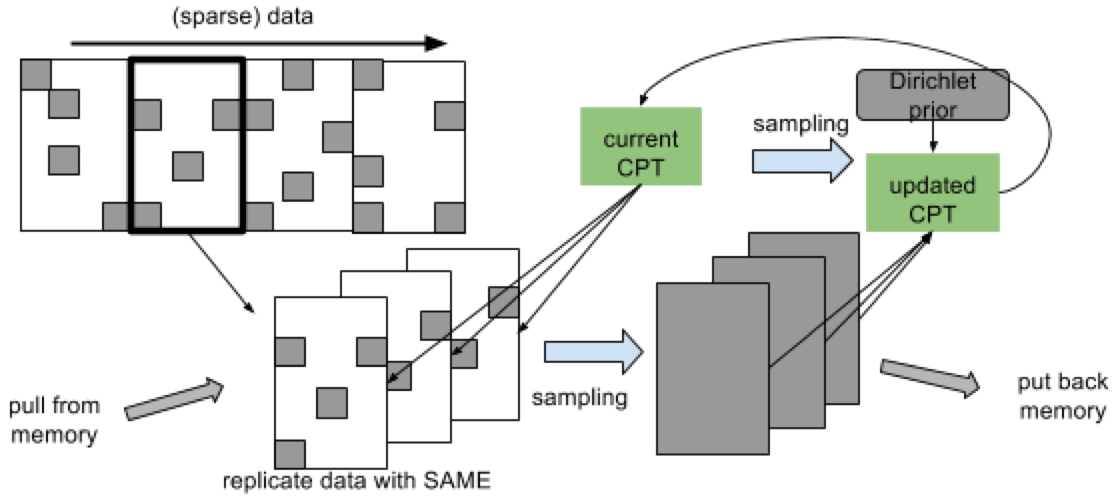
\includegraphics[width=0.8\textwidth]{fig_BIDMach_flow_DRAFT}
\caption{\textbf{TODO I think having a short, fat BIDMach visualization would be great, but it needs
to be publication quality.} This is a visualization of our Gibbs sampler. It takes in sparse data,
replicates it using SAME (with $m=4$ here), samples them (using the same set of CPTs), then uses
those samples, along with the prior and the current CPT to estimate the new CPT.}
\label{fig:BIDMach}
\end{figure}

Figure~\ref{fig:BIDMach} shows a visualization of how our Gibbs sampler works. It is implemented and
integrated as part of the open-source BIDMach library~\citep{bidmach} for machine learning. Our
Gibbs sampler expects a data matrix, where typically, rows represent variables and columns represent
cases. BIDMach divides data into ``mini-batches'' and iterates through batches sequentially, and
going through all mini-batches is considered one full pass over the data.

For each mini-batch, our sampler will form $m$ copies of the data, where $m$ is the SAME parameter,
and where the known data is kept the same across all copies. Then, it performs Gibbs sampling to
fill in the unknown values in each copy of the mini-batch using the same set of CPTs.  These sampled
results are combined with an adjustable Dirichlet prior and (if desired) the current
CPT\footnote{This would be useful if one wanted to do a moving average'' update of the CPT. Also,
the use of the Dirichlet prior tends to be more important when the data is sparse, since it
``smooths'' the CPTs.} to form a set of discrete counts that we then sample from to estimate the
updated CPT. We then proceed to the next mini-batch of data and peform Gibbs sampling on that using
the new CPT. To preserve samples across all runs, each time we finish a mini-batch, we store the
sampled results in memory. Then, during the next \emph{pass} over the data (i.e., after having gone
through all the mini-batches) we start the Gibbs sampling process from data that we load from
memory.

There are many ways that we optimize the sampler to maximize throughput on one computer and to avoid
memory allocation errors. First, our sampler is GPU accelerated and takes advantage of parallelism
in SIMD hardware by implementing the sampling process using matrix operations. In fact,
in~\citep{SAME2015}, they found that multinomial sampling was one of the bottlenecks, but we
implement multinomial sampling using straightforward matrix operations.

Since memory on GPUs are scarce, we use a matrix caching strategy to reuse memory for same-sized
matrices. This is also the reason why we use mini-batch updates, since the updates are all of the
same size and so the matrices that result from a mini-batch have the same container and thus we
re-use their memory slots\footnote{This does not generally apply to the very last mini-batch, but
that last batch would not cost too much in extra memory, and one can even ignore it if needed}. The
settings we use are customizable, so one can reduce the mini-batch size to reduce the memory
footprint. One needs to do this step to perform SAME sampling with high $m$, since more replication
takes up more memory.

\textbf{TODO Integrate this!}

Early attempts at speeding up Gibbs sampling explored extents to which it could be parallelized.
Gibbs sampling is a sequential algorithm and cannot be completely parallelized, but it is possible
to exploit conditional independence assumptions to perform certain sampling steps simultaneously.
The idea is to apply graph coloring to the moralized graph  $\tilde{\mathcal{G}}$ of the network.
One property of Bayesian networks is that $u, v \in \mathcal{V}$ are independent conditioning on a
set of variables $\mathcal{C}$ if $\mathcal{C}$ includes at least one variable on every path
connecting $u$ and $v$ in $\tilde{\mathcal{G}}$. That is, vertex set $\mathcal{C}$ separates the
dependency between $u$ and $v$.

Assume there is a $k$-coloring of $\tilde{\mathcal{G}}$ such that each vertex is assigned one of $k$
colors and adjacent vertices have different colors. Denote $\mathcal{V}_c$ the set of variables
assigned color $c$ where $1 \leq c \leq k$. One can sample sequentially from $\mathcal{V}_1$
to $\mathcal{V}_k$, where within each color group, it samples all the variables in parallel. This
parallel sampler corresponds exactly to the execution of a sequential scan Gibbs sampler for some
permutation over the variables~\citep{Gonzalez2011}. That is, the algorithm will converge to the
desired distribution because (intuitively) variables within one color group are independent to each
other given all the other variables. Finding the optimal coloring of a graph is NP-complete in
general, but efficient heuristics for balanced graph coloring perform well in many real word
problems.

\textbf{Actually, the above really should be in Section 4! Then I have to think about what
appropriate related work would be like.}



\section{Experiments}\label{sec:experiments}

We test our Gibbs sampler on one synthetic and one real dataset.  We compare our Gibbs sampler with
JAGS~\citep{JAGS2003}, which is the most popular and efficient tool for Bayesian inference. JAGS is
the fairest comparison to our sampler because it uses Gibbs sampling as the primary inference
algorithm. There are alternative ways of estimating CPTs, but most of them (e.g., STAN, Bayes Net
Toolbox) lack the support of efficient inference of discrete models, and are not included in the
benchmarks.

Our sampler and JAGS are evaluated on a PC equipped with a single 4-core CPU (Intel Core i7-3667U)
and a dual-core GPU (Nvidia GTX-690). Only one core of GPU is used in the benchmark. We also use
Intel VTune Amplifier to profile each program and measure the flops performance. VTune is very power
tool: It allows user to attach any running process and monitor the all the hardware instructions
executed, including both X87 legacy floating point operations and SSE operations.  We emphasize that
the use of one computer is deliberate, as it is cheaper and simpler to use as compared to a
computing cluster.

\textbf{TODO The above is for stout, I think. We need the updated specs for bitter.}

\subsection{Synthetically Generated Student Data}\label{ssec:student_data}

% TODO It might be tricky to get the DAG resized correctly so that the figures line up nicely.
\begin{figure}[t]
  \centering
  \begin{minipage}{.46\textwidth}
    \centering
    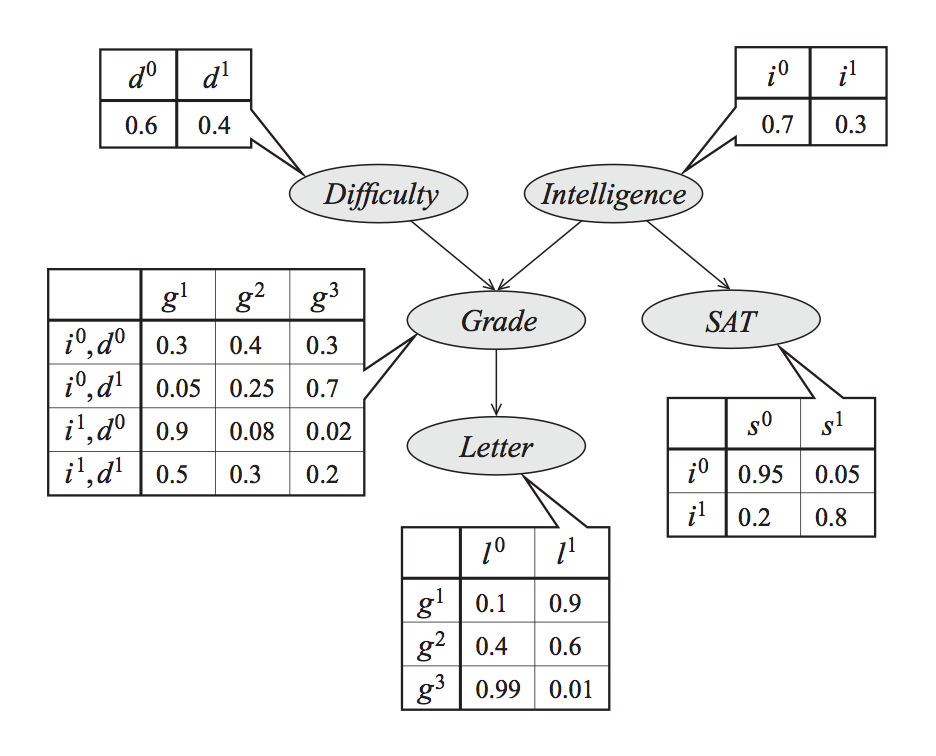
\includegraphics[width=1\textwidth]{fig_student_diagram}
    \caption{The student data.}
    \label{fig:student_diagram}
  \end{minipage}\hfill
    \begin{minipage}{.5\textwidth}
    \centering
    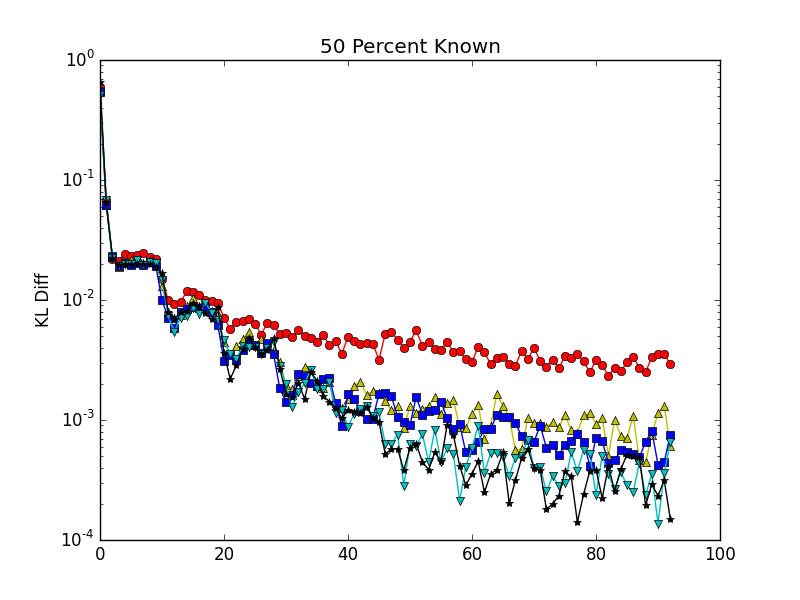
\includegraphics[width=1\textwidth]{fig_kl_student_50perc}
    \caption{Average KL divergence.}
    \label{fig:kl_accuracy}
  \end{minipage}
\end{figure}

We use synthetic data generated from a toy Bayesian network to illustrate proof of correctness and
other concepts. Figure~\ref{fig:student_diagram} shows the network we are using,
from~\citet{koller2009}. The goal is to model a student taking a class, with metrics of skill
(Intelligence and SAT score), the class difficulty, and the student's resulting grade, which
subsequently affects the quality of a letter of recommendation.

To generate the data, we performed direct sampling on a topological ordering of the variables with
$X_0 = {\rm Intelligence}$, $X_1 = {\rm Difficulty},$ $X_2 = {\rm SAT}$, $X_3 = {\rm Grade}$, and
$X_4 = {\rm Letter}$. Variable $X_i$ gets sampled according to the values of its parents (if any)
based on the true distribution from Figure~\ref{fig:student_diagram}. We generated one million
samples, which means our data is formatted in a $(5\times 10^6)$-dimensional matrix. Then, we
randomly hid 50\% and 75\% of the data to form two respective datasets. The goal is to use the
remaining known data, and to use Gibbs sampling, to sample the unknown values, and then those
determine the next sample of the CPT. The objective is to estimate the resulting set of CPTs to see
if they match the ones from Figure~\ref{fig:student_diagram}.

There are several metrics of measuring how well our sampler converges. The one we use is the average
Kullback-Liebler divergence $KL_{\rm avg}$. For two distributions $p(x)$ and $q(x)$, the
KL-divergence is $\sum_x p(x) \log(p(x)/q(x))$ where we iterate over $x$ such that $q(x) > 0$. Since
the set of CPTs has multiple probability distributions (e.g., the ``Grade'' variable ``contributes''
four probability distributions), we must consider all of them. In this data, there are eleven CPTs,
so the ``average KL divergence'' metric we use is

% Daniel: NOTE we could put this earlier in section 5, and define it better b/c we also use it in
% section 5.2.
\begin{equation}\label{eq:avg_kl}
KL_{\rm avg} = \frac{1}{11}\sum_{i=1}^{11} p_i(x) \log\left(\frac{p_i(x)}{q_i(x)}\right).
\end{equation}

Notice that for all $i$, $p_i(x)$ represents the corresponding \emph{true} distribution, and
$q_i(x)$ is what our sampler estimates. Our sampler will sample the missing values, and then use
those counts along with a Dirichlet prior to form a new Dirichlet distribution, which we then sample
from to form the next (ideally, improved) estimate of the true set of CPTs. We use a uniform
Dirichlet prior with all ones for simplicity.

Figure~\ref{fig:kl_accuracy} plots the $Kl_{\rm avg}$ for both versions of the student data (on a log
scale). For each version, we use four different SAME parameters, $m = \{1,5,10,50\}$. Our results
show that, intuitively, the sampler can better converge to the true CPT with more known data (50\%
known in our case). In addition, increasing $m$ results in CPT estimates that more closely match the
true CPTs, though there are diminishing returns, as the increase from $m=1$ to $m=2$ results in a
similar performance improvement as an increase from $m=2$ to $m=50$. To put our $KL_{\rm avg}$
metric in perspective, when $m=50$, the sampler is accurate to the true CPTs by around three
significant figures. \textbf{TODO: this figure needs the results from the 25\% data, and we need to
make it cleaner, but otherwise that is the main idea.}

Next, we evaluate how the SAME parameter $m$ affects the overall runtime of the sampler, since more
samples means the algorithm runs longer.  Figure~\ref{fig:kl_time} plots the average KL divergence
(on a log scale) versus the time, measured in seconds, for SAME parameters $m = \{1,5,10,20,50\}$ on
the 25\% known data (the 50\% known data had similar results). Each ``point'' in the graph (i.e.,
the shapes that are connected via edges) represents the $KL_{\rm avg}$ measured at the end of a pass
over the data over one mini-batch. We see that larger $m$ results in longer runtimes per pass, since
the curve for $m=1$ has points closer together as compared to $m=5$, and so on. The curves for some
of the smaller values of $m$ were not improving substantially after the first set of iterations,
which is why they are not extended as far in the graph. Note that the graph for $m=50$ has a
starting point that is after the other curves, indicating that higher $m$ means a larger initial
startup time (as expected). But as the curve proceeds, it only takes about 25 seconds before the
largest $m$ provides a superior time-accuracy tradeoff. Before that, $m=10$ and $m=20$ appear to be
better.

We conclude that for the $m$ values we test, increasing $m$ results in better accuracy per time
after only a few passes through the data, so there is substantial benefit to SAME sampling. (In
Section~\ref{sec:discussion}, we discuss the time-versus-$m$ tradeoff in more detail.)

\begin{figure}[t]
  \centering
  \begin{minipage}{.5\textwidth}
    \centering
    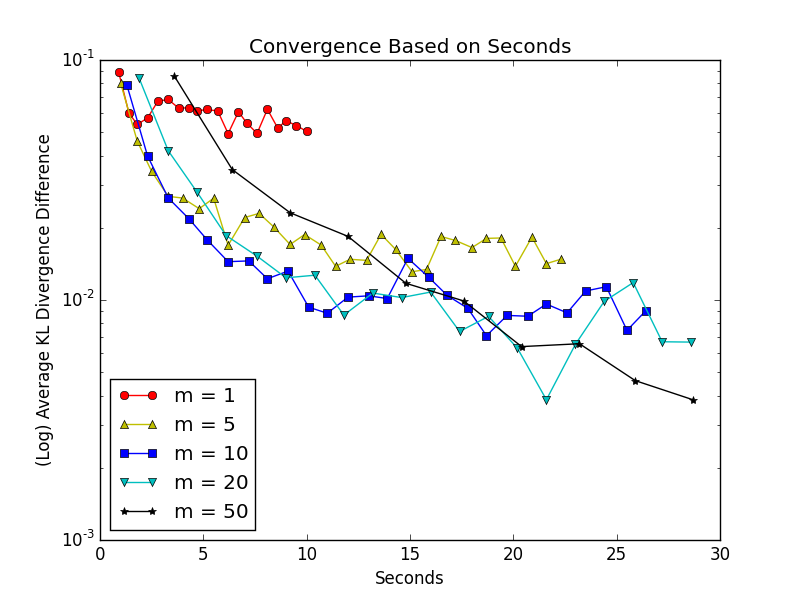
\includegraphics[width=1\textwidth]{fig_kl_time_log}
    \caption{Accuracy versus time.}
    \label{fig:kl_time}
  \end{minipage}\hfill
    \begin{minipage}{.5\textwidth}
    \centering
    \fbox{\rule[-.5cm]{0cm}{4cm} \rule[-.5cm]{4cm}{0cm}}
    %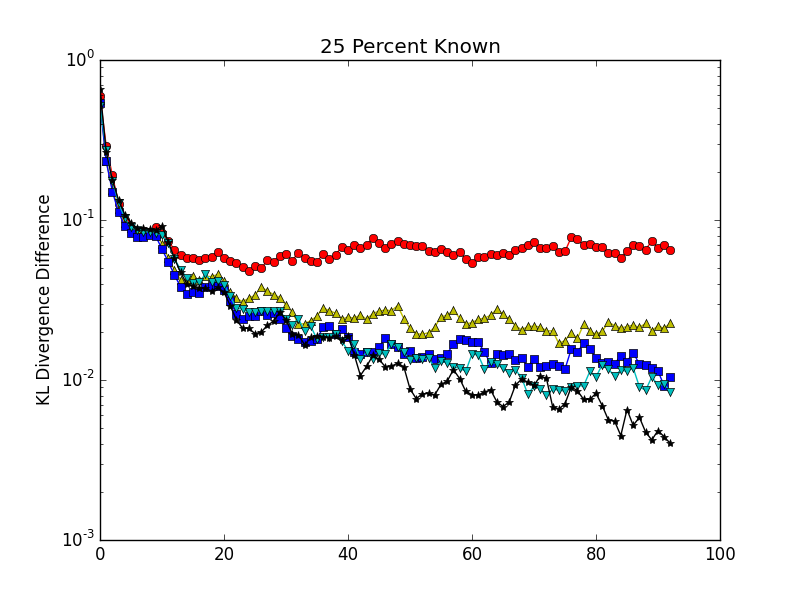
\includegraphics[width=1\textwidth]{fig_kl_student_25perc}
    \caption{Consecutive CPT convergence.}
    \label{fig:consecutive_cpts}
  \end{minipage}
\end{figure}

Finally, we also test another way of measuring convergence, which is the average KL divergence
applied to CPTs produced by our sampler on consecutive passes over the data. Thus, instead of
comparing with the true probability distributions, we are comparing the distributions our sampler
estimates. These are shown in Figure~\ref{fig:consecutive_cpts}, which indicates that with higher
$m$ values, the algorithm is quicker to converge to a set of parameter estimates (which themselves
are higher quality, based on Figure~\ref{fig:kl_accuracy}).

It should also be noted that we benchmarked this with JAGS, which also obtains the true CPTs. JAGS,
however, cannot run on the entire million of samples in a reasonable amount of time. It took one
hour for JAGS to run on just 10000 variables. \textbf{TODO Yeah, I think we need to have solid
benchmarks here, and I can cut back on some of the other earlier stuff.}.

\subsection{Real Dynamic Learning Maps ``MOOC'' Data}\label{ssec:mooc_data}

We now benchmark our code on a Bayesian network with a nation-wide examination dataset from the
Dynamic Learning Maps (DLM) project. The dataset contains the assessment (correct or not) of 30,000
students' responses to questions from the DLM Alternate Assessment System. There are 4000 students
and 340 unique questions in the pilot experiment, and the overall completion rate of the questions
is only 2.2\% (assessment questions are tailored for each student). Each of the 340 questions is
considered to be derived from a set of 15 basic concepts, and relations between questions and
concepts and within concepts are given in the DAG file, which we will specify later.  Each question
is considered as a observed node in the Bayesian network, with a very high missing value rate, and
each concept is considered as a hidden node which never gets observed. Each node is binary-valued.
The inference task is to learn the parameter of the network on 80\% of the response assessment and
predict on the rest 20\% of the response.

After data preprocessing, we have our data as a $(334 \times 4367)$-dimensional matrix, where there
are 334 variables and 4367 students. The first 15 variables are latent and never observed across all
students, and they form the set of parents for the remaining 319 variables. Only 2.2 percent of the
data is known, so the data is extremely sparse.

We evaluate our sampler using two methods. The first is the consecutive KL divergence difference
from Figure~\ref{fig:consecutive_cpts}. The second is the prediction accuracy to measure the quality
of the model, which we did not use to evaluate the five-variable student data. As before, we also
benchmark our sampler with JAGS.

Figure~\ref{fig:mooc_cpts} shows the consecutive KL divergences across consecutive iterations. We
see that higher $m$ values result in better convergence. \textbf{TODO Well, we have to do this one
first.}

%\subsection{Performance and Runtime}
%We first look at the efficiency of each system measured by giga floating point operations per second
%(Gflops). Intel VTune Amplifier is used to measure the flops numbers. As presented in Figure
%\ref{perf}, BIDMach achieves 5 Gflops and 1 Gflops for GPU and CPU respectively. The Gibbs sampler
%is bottlenecked by the calculation of sampling probability vectors which is implemented using SpMV
%operations. Such flops numbers are the hardware limit of SpMV operation. Jags and Infer.net operates
%at much lower flops rates. Note that the y-axis of the figure is in log-scale. The VTune profile
%results also show that Jags spend 70 \% of the runtime on disk IO, which is highly inefficient. We
%also observe that the memory usage of Infer.net is not efficient: on our PC with 8G memory, it
%cannot scale up to 10000 students (with the same statistics as the DLM pilot dataset we use).

Next, we use prediction accuracy. For each node to be predicted, we sample 50 instances for that
node from the learned network and observed values, and then take the majority as the predicted
value. The accuracy is measured as the percentage of corrected predictions.
Figure~\ref{fig:mooc_accuracy} shows the accuracy results.  \textbf{TODO I would like to do this,
and I think this is important. We should be seeing that accuracy goes up to about 66\%.
Unfortunately, the actual data is skewed in a 66\% to 33\% ratio so ... let me figure out if I can
spin that positively.}

\begin{figure}[t]
  \centering
  \begin{minipage}{.5\textwidth}
    \centering
    \fbox{\rule[-.5cm]{0cm}{4cm} \rule[-.5cm]{4cm}{0cm}}
    %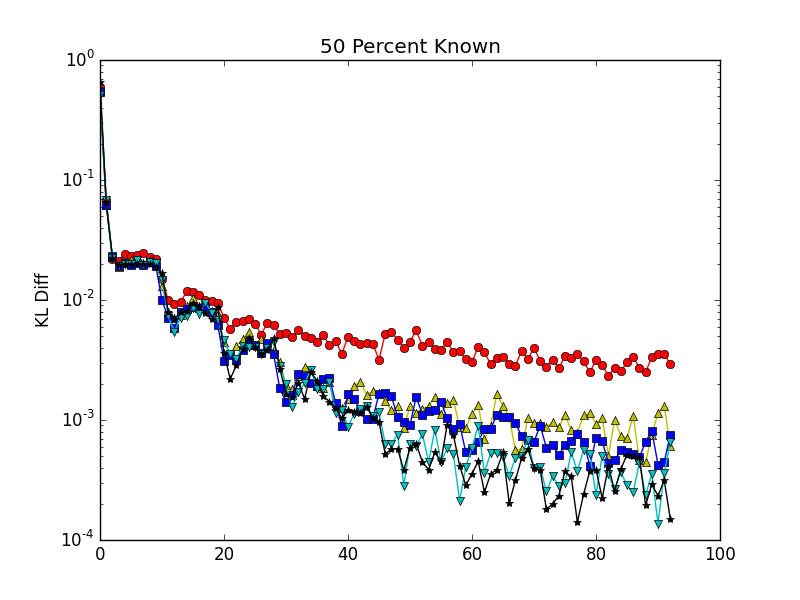
\includegraphics[width=1\textwidth]{fig_kl_student_50perc}
    \caption{\textbf{MOOC Convergence}}
    \label{fig:mooc_cpts}
  \end{minipage}\hfill
    \begin{minipage}{.5\textwidth}
    \centering
    \fbox{\rule[-.5cm]{0cm}{4cm} \rule[-.5cm]{4cm}{0cm}}
    %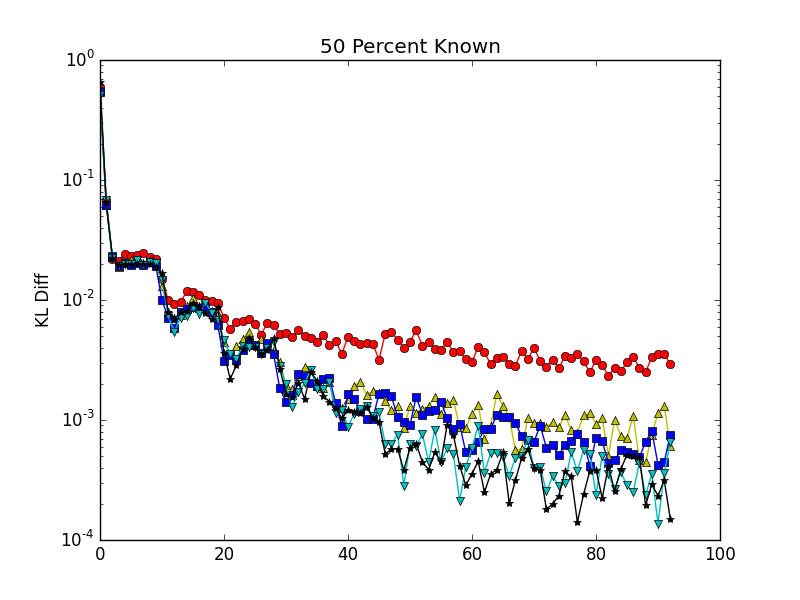
\includegraphics[width=1\textwidth]{fig_kl_student_50perc}
    \caption{\textbf{MOOC ``Accuracy''}}
    \label{fig:mooc_accuracy}
  \end{minipage}
\end{figure}

We emphasize that in terms of runtime, BIDMach is easily able to run this data. In all, it takes
about ten seconds to run Gibbs sampling through this data, whereas JAGS takes hours. In fact, the
main thing that is holding our algorithm back is the limited memory of GPUs, which means we need to
shrink the batch size with large $m$. As memory on GPUs becomes cheaper, we will be able to run
Gibbs sampling and perform graphical model inference on larger datasets. \textbf{Again, we should
formalize the JAGS comparisons.}




\section{Discussion}\label{sec:discussion}

One interesting thing about the experiments is the contribution of SAME to Gibbs sampling.  Table
(???) shows the time performance and gigaflops of BIDMach on various settings. One can see that
increasing $m$ for $m < 50$ results in steady gflops increases but \emph{without} an equivalent
increase in time. Then, once $m$ gets large, SAME ``saturates'' and the runtime increases while the
gflops stalls. This matches the results from~\citep{SAME2015} and argues for the importance of
testing with a variety of $m$ values.

% This table will be for SAME stuff
\begin{table}[t]
\caption{Sample table title (Perhaps we can list JAGS/BIDMach runtime here?)}
\label{sample-table}
\begin{center}
\begin{tabular}{ll}
\multicolumn{1}{c}{\bf PART}  &\multicolumn{1}{c}{\bf DESCRIPTION}
\\ \hline \\
Dendrite         &Input terminal \\
Axon             &Output terminal \\
Soma             &Cell body (contains cell nucleus) \\
\end{tabular}
\end{center}
\end{table}

\textbf{TODO more detailed discussion of SAME and runtime/gflops. Perhaps also discuss memory usage
(as I do earlier)? Not else sure what to put here, but I'm not sure if we want to increase the
experimental section of this paper yet again with this stuff.}

\section{Conclusions}\label{sec:conclusions}

We conclude that SAME Gibbs sampling using our sampler is much faster than the state of the
art (JAGS) in Gibbs sampling, and also that it is fast enough to apply to data with several hundreds
of variables. We argue that SAME Gibbs sampling should be the method researchers use to perform
inference on such Bayesian networks. Future work will explore the application of our sampler to a
wider class of real-world datasets.


\subsubsection*{Acknowledgments}

We thank Biye Jiang and Huasha Zhao for helpful discussions. Daniel Seita is supported by the
Berkeley and National Physical Science Consortium Fellowships.

% TODO Yeah make the references section a *lot* cleaner!
\bibliography{iclr2016_conference}
\bibliographystyle{iclr2016_conference}










%% APPENDIX
\clearpage
\appendix

\section{Random Appendix Stuff}

\textbf{I expect that we will use eight pages for text, plus the ninth page for references. Then the
remaining material (if any) will go here.}









% Daniel: all of this stuff is older material ...
\begin{comment}
\section{Mathematical Details}

Going back to our inference problem, sampling all variables in a color group can be formulated into
matrix operations. To sample any unobserved $u \in \mathcal{V}$ using Gibbs sampling, we need to
compute $f_u(X_u = i) = \log P(X_u = i \mid X_{\mathcal{V} \setminus \{u\}})$ for all $i$ in the
support of $X_u$. Notice that we are using $X_u = i$ as the argument to make it clear what value
$X_u$ is taking on.

To find $f_u(X_u = i)$, we can evaluate them as follows:
\begin{equation}\label{eq:parameter}
f_u(X_u = i) = \theta_{X_u=i \mid \pi_u} + \sum\limits_{v \in \xi_u} \theta_{X_v \mid \pi_v} + C_2,
\end{equation}
where $C_2$ is a constant that does not depend on the value (i.e., state) of $X_u$, and $\xi_u$
denotes the set of children of $X_u$. Because we are sampling from $X_u$, we will assume that all
other variables $X_{\mathcal{V}\setminus \{u\}}$ are assigned a known value (either from data, or
from a Gibbs sampling assignment), so for instance, $\pi_u$ in Equation~\ref{eq:parameter} really
denotes $\{X_{p_1} = k_1, \ldots, X_{p_n} = k_n\}$ where $n$ is the size of $\pi_u$. Furthermore, be
aware that for the summations, the assumption that $X_u = i$ is embedded in all the $\pi_v$ sets,
since $X_i \in \pi_v$. For details on the derivation, see Appendix~\ref{app:math}.

Once we have $f_u(X_u = 0), \ldots, f_u(X_u = k)$ for $X_u$, how do we sample from it? We simply
exponentiate all these terms to get the following vector:
\[
\begin{bmatrix}
\exp \left(\theta_{X_u=0 | \pi_u} + \sum_{v \in \xi_u} \theta_{X_v\mid \pi_v} + C_2\right) \\
\exp \left(\theta_{X_u=1 | \pi_u} + \sum_{v \in \xi_u} \theta_{X_v\mid \pi_v} + C_2\right) \\
\cdots \\
\exp \left(\theta_{X_u=k | \pi_u} + \sum_{v \in \xi_u} \theta_{X_v\mid \pi_v} + C_2\right) 
\end{bmatrix}
=
\begin{bmatrix}
\exp \left(\theta_{X_u=0 | \pi_u} + \sum_{v \in \xi_u} \theta_{X_v\mid \pi_v}\right) \\
\exp \left(\theta_{X_u=1 | \pi_u} + \sum_{v \in \xi_u} \theta_{X_v\mid \pi_v}\right) \\
\cdots \\
\exp \left(\theta_{X_u=k | \pi_u} + \sum_{v \in \xi_u} \theta_{X_v\mid \pi_v}\right) 
\end{bmatrix}
e^{C_2},
\]
and dumping the $e^{C_2}$ term gives us the un-normalized probability vector for $X_u$ taking on any
of its possible values given the value of all other nodes in the graph. It's probably easiest to
think about sampling from a vector in terms of ranges, so if our probability vector was $[0.4 \quad
0.5 \quad 0.1]$, then we could sample $X_u$ from a uniform random variable $ x \in [0,1]$. If $x \in
[0,0.4]$, we assign 0, if $x \in [0.4, 0.4+0.5]$, we assign 1, and if it exceeds $0.9$ we assign 2.

\subsection{Matrix Formulation and Code Details}

Algorithm~\ref{alg:PBI} shows a parallel Bayesian Network inference algorithm that uses matrix
operations to conduct sampling. It is approximate in the sense that while the general idea is right,
there are still many special cases or details not covered here for the sake of clarity.

\begin{algorithm}
\caption{Parallel BayesNet Inference}
\begin{algorithmic}[1]
\State $A =$ adjacency matrix of graph $\mathcal{G}$
\State Initialize the conditional probability table (CPT) with random values, and then normalize
\State $B =$ local encoding matrix of $\Theta$
\State $C =$ global offset vector of $\Theta$
\State Initialize the network $X^1_{\mathcal{V}}$: random for unobserved nodes, fixed for observed nodes
\For{ $t=1 \to t_{max}$}
\For{ $c=1 \to k$}
\State Set $maxStates$ to be the maximum number of states of all variables in $\mathcal{V}_c$.
\For{ $i=0 \to maxStates-1$}
\State Set $\mathcal{C}_i$ to be the set of variables that have nonzero probability of attaining $i$.
\State $Y^i =$ set $(X^t_{\mathcal{C}_i} = i)$ for variables in $X^t_{\mathcal{C}_i}$, random otherwise.
\State $\phi^i = \text{$\theta$-lookup} (C + B \times Y^i ) $
\State $A_{\mathcal{C}_i} = (A + I)_{\mathcal{C}_i, \mathcal{C}_i \cup \xi_{\mathcal{C}_i}}$
\State $P^i = \exp\left(A_{\mathcal{C}_i} \times \phi^i\right)$
\EndFor
\State Sample $Z_{\mathcal{V}_c}$ uniformly (from [0,1]) at random
\State Using $Z_{\mathcal{V}_c}$, and all of the $P^i$ computed earlier, sample $X^{t+1}_{\mathcal{V}_c}$ in parallel
\State Update the CPT
\EndFor
\EndFor
\end{algorithmic}
\label{alg:PBI}
\end{algorithm}

Let's analyze Algorithm~\ref{alg:PBI} carefully. Before we begin the Gibbs sampling iteration, we need
to do several things:

\begin{itemize}
    \item We need the adjacency matrix $A$ of the graph. $A$ has a 1 at index $(i,j)$ if there is an
    edge from node $X_i$ to node $X_j$, and 0 otherwise. Thus, a column of the adjacency matrix at
    index $j$ will reveal all of $X_j$'s parents.
    \item We need to set up the conditional probability table (CPT) which can collectively be viewed
    as $\Theta$. This is internally stored as a single array, where each element corresponds to one
    instance of a conditional probability, $P(X_i = k_0 \mid X_{p_1} = k_1, \ldots, X_{p_n} = k_n)$,
    where $X_{p_1}, \ldots, X_{p_n} \in \pi_i$. To enable efficient indexing and lookups, we
    consider the CPT construction according to a topological ordering of the variables. Thus, if
    $X_1$ represents the first node, then the CPT starts with $P(X_1 = k \mid \pi_1)$ for all $k$
    candidates\footnote{Of course, in this case, $\pi_1 = \emptyset$.}. Then once those
    possibilities have occurred, the table moves on to $P(X_2 = k \mid \pi_2)$, and so on. In other
    words, each variable $X_i$ occupies a contiguous block in the CPT, where the block is defined by
    all choices of $P(X_i \mid \pi_i)$ for these variables\footnote{This construction assumes that
    we have a way of knowing the number of possible states for each variable. This seems like a weak
    assumption, and if it is not true, then one can resolve this by looking through the entire data
    to construct the state set for each variable.}.
    \item For fast lookups, we need the local encoding matrix $B$ of the variables. In our code, we
    name this matrix \texttt{iproject}. This matrix is designed to take advantage of how we order
    the variables in the CPT. While it is clear that we order $P(X_i\mid \pi_i)$ based chiefly on
    the index of $i$, we \emph{also} have to carefully order the CPT based on the \emph{parent}
    assignments! We choose an assignment where the parent with index closest to the current node of
    interest gets changed first, and this proceeds recursively until the first parent. This results
    in \texttt{iproject} being a lower triangular matrix with ones on the diagonal, and for each
    row, as one ``moves left'' (i.e., the column index becomes smaller) values are either 0 or are
    multiplicatively increasing compared to the most recent nonzero element. The exact details of
    this are not too difficult to understand once one has thought through it carefully, but for
    space reasons we decide to omit our exact construction.
    \item Also for fast lookups, we need the global offset vector $C$ of the variables. This is a
    single column vector where $C[i]$ indicates the starting index in the CPT where variable
    $X_i$ starts its contiguous block. (Or $X_{i+1}$, depending on how one chooses to start one's
    indexing scheme.)
\end{itemize}


Once the initialization has concluded, we loop through the number of iterations, and within each
iteration, we loop through the color groups so that we can sample those in parallel. It now remains
to show how we can efficiently sample one color group.

Suppose we are in a color group specified by the set $\mathcal{V}_c$. In general, the variables in
this set will not all have the same number of possible states. One might be a binary variable (two
states), another might have five states, and so on. We set $maxStates$ to be the maximum over all
the state possibilities of each variable. Then we loop through $i = \{0, 1, \ldots, maxStates-1\}$,
and for each iteration, we extract a set $\mathcal{C}_i \subseteq \mathcal{V}_c$ of variables that
can take on state $i$. Since we assume all variables have states $\{0,1,...,k\}$, this means for
$i=0$ and $i=1$, $\mathcal{C}_i = \mathcal{V}_c$. The reason for doing this is that we define $Y_i$
to be a column vector\footnote{In reality, this is not usually true, but it is easiest to start out
by thinking this way.} whose value is $i$ for all nodes in $\mathcal{C}_i$, and it does not make
sense to assign $i$ to a node that cannot ever obtain that state. Note that $Y^i$ has the same
number of rows as nodes (thus we use ``row'' and ``node'' interchangeably), so aside from those
nodes in $\mathcal{C}_i$, the other nodes are assigned randomly.  For a binary random variable, it's
randomized between 0 and 1, equally distributed. For a ternary, it's randomized between 0, 1, and 2
equally, and so on.

Once we have $Y^i$s, then we can compute intermediate terms that correspond to model parameters in
$\Theta$. This involves $C + B\times Y^i$ because this will index into the appropriate spots in the
CPT. The resulting column vectors $\phi^i$ are such that they will provide the $P(X_u = i \mid
\pi_u) = \theta_{X_u = i \mid \pi_u}$ parameters for those nodes that can actually attain the state
$i$. Keep in mind that the values these variables are assigned to is based only on the current
configuration, which we recall was randomly assigned other than $X_u = i$.

The next step is to compute the actual probability $P(X_u = i \mid X_{\mathcal{V}\setminus \{u\}})$,
which we computed in Equation~\ref{eq:parameter}. This involves a simple matrix multiplication:
$A_{\mathcal{C}_i} \times \phi^i$. That matrix multiplication works by summing through terms in a
row of the first matrix and a column of the second matrix will result in the $\theta_{X_u\mid \pi_u}
+ \sum_{v\in\xi_{u}} \theta_{X_v\mid \pi_v}$ terms that are familiar to us. Incidentally, we obtain
$A_{\mathcal{C}_i}$ from $A$ (which in the code is named \texttt{pproject}) by taking only a subset
of the rows and a subset of the columns, similar to how slicing operations works. It comes from
$A_{\mathcal{C}_i} = (A + I)_{\mathcal{C}_i, \mathcal{C}_i \cup \xi_{\mathcal{C}_i}}$, which means
we first start with the dag plus the identity, then extract all rows corresponding to indices of
this color group satisfying the ``existence of state $i$ requirement,'' then only keep the columns
corresponding to those nodes, plus their children, which is where we get the $\sum_{v\in \xi_{u}}$
part. It is also necessary to slice $\phi^i$ to make the matrix multiplication eligible.

At the end of all this, just before moving on to the next color group, we finally sample. For the
sake of brevity, the sampling process itself is described informally in Algorithm~\ref{alg:PBI}. We
point out that our sampling, as well as most other procedures in this algorithm, is done in matrix
operations, which fully utilizes the parallelism provided by the hardware.

In a footnote earlier, we mentioned that $Y^i$ is not actually a column vector in our code. To
increase parallelism in practice, we instead have matrices we call \texttt{statei} where each column
is like its own $Y^i$, but the unknown values will be randomly assigned. This allows us to
effectively sample multiple observations in a single batch. In particular, for the dataset we use,
these ``multiple observations'' correspond to ``multiple students.''

\section{Derivation of Log Probabilities}\label{app:math}

In this section, we derive Equation~\ref{eq:parameter} to determine $f_u(X_u=i)$. For simplicity, we
dump the $i$ in the following computation. We assume that $X_u$ is in color group $\mathcal{V}_c$.
\begin{align}
f_u(X_u) &= \log P(X_u | X_{\mathcal{V} \setminus \{u\}}) \\
    &\stackrel{\text{(1)}}{=} \log P(X_u | X_{\mathcal{V} \setminus \mathcal{V}_c}) \\
    &\stackrel{\text{(2)}}{=} \log P(X_u, X_{\mathcal{V} \setminus \mathcal{V}_c}) + C_1 \\
    &\stackrel{\text{(3)}}{=} \log \left( \sum\limits_{ \mathcal{V}_c \setminus \{u\}}\prod\limits_{v \in \mathcal{V}} P(X_v | \pi_v) \right) + C_1  \\
    &\stackrel{\text{(4)}}{=} \log \left( P(X_u | \pi_u) \prod\limits_{v \in \xi_u} P(X_v | \pi_v) \times \sum\limits_{ \mathcal{V}_c \setminus \{u\}}\prod\limits_{v \in \mathcal{V} \setminus (\xi_u \cup \{u\})} P(X_v | \pi_v) \right) + C_1 \\
    &\stackrel{\text{(5)}}{=} \log P(X_u | \pi_u) + \sum\limits_{v \in \xi_u} \log P(X_v | \pi_v) + C_2 \\
    &\stackrel{\text{(6)}}{=} \theta_{X_u | \pi_u} + \sum\limits_{v \in \xi_u} \theta_{X_v | \pi_v} + C_2.
\end{align}

Stage (1) is true by the dependency encoded in the network and the construction of the coloring.
Stage (2) comes from Bayes' rule, where $C_1$ is a constant that does not depend on the state of
$X_u$. Stage (3) expands the marginal distribution by definition; we have a joint distribution over
a subset of the variables, so we must sum out the variables that do not appear in the joint.

Stage (4) is a critical step for the matrix formulation. Let $\xi_u$ be the children set
of node $u$. By the construction of the graph coloring, a key observation is that
\begin{align}
(\{u\} \cup \pi_u \cup \xi_u \cup \pi_{\xi_u}) \cap (\mathcal{V}_c \setminus \{u\}) = \emptyset. 
\label{ind}
\end{align}
That is, node $u$, its parents, its children and the parents of all its children have no intersect
with any nodes in the color group except $u$ itself. This allows us to take out the term $\log P(X_u
| \pi_u) \prod\limits_{v \in \xi_u} P(X_v | \pi_v)$ from the summation, and gives us a factorized
form of the marginal distribution.

Stage (5) rearranges $\log$ and product terms. $C_2 = C_1 + \sum\limits_{ \mathcal{V}_c \setminus
\{u\}}\prod\limits_{v \in \mathcal{V} \setminus (\xi_u \cup \{u\})} P(X_v | \pi_v)$ which again does
not depend on $X_u$, and finally (6) plugs in the definition of $\theta$.

Now that we have $f_u(X_u = i)$ for all possible states $i$, it remains to show how to actually
sample. If $X_u$ were binary, then it would be simple because then we could just evaluate the
following ratio:
\begin{equation}
\alpha_u = {e^{(f_u(0)-f_u(1))}} = {e^{(g_u(0)-g_u(1))}} ,
\end{equation}\label{alpha}
where $g_u(X_u) = \theta_{X_u | \pi_u} + \sum\limits_{v \in \xi_u} \theta_{X_v | \pi_v}$ and $C_2$
is canceled out, which makes sense as it is effectively a normalizing constant. As a sanity check,
the sampling of $X_u$ does not depend on the assignments of any other variables in the same color
group by Equation \ref{ind}.






% Daniel: I'm leaving this here for now, because this is some extra stuff from Huasha's old write-up
% that we might use.

We benchmark all the systems on fitting a Bayesian network with a nation-wide examination dataset
from the Dynamic Learning Maps (DLM) project. The dataset contains the assessment (correct or not)
of 30,000 students' responses to questions from the DLM Alternate Assessment System. There are 4000
students and 340 unique questions in the pilot experiment ,and the overall completion rate of the
questions is only 2.2 \% (assessment questions are tailored for each student). Each of the 340
questions is considered to be derived from a set of 15 basic concepts, and relations between
questions and concepts and within concepts are given. Each question is considered as a observed node
in the Bayesian network (with very high missing value rate), and each concept is considered as a
hidden node which never gets observed. Each node takes a binary value. The inference task is to
learn the parameter of the network on 80\% of the response assessment and predict on the rest 20\%
of the response. We use the prediction accuracy to measure the quality of the model. 

\subsection{Performance and Runtime}
We first look at the efficiency of each system measured by giga floating point operations per second
(Gflops). Intel VTune Amplifier is used to measure the flops numbers. As presented in Figure
\ref{perf}, BIDMach achieves 5 Gflops and 1 Gflops for GPU and CPU respectively. The Gibbs sampler
is bottlenecked by the calculation of sampling probability vectors which is implemented using SpMV
operations. Such flops numbers are the hardware limit of SpMV operation. Jags and Infer.net operates
at much lower flops rates. Note that the y-axis of the figure is in log-scale. The VTune profile
results also show that Jags spend 70 \% of the runtime on disk IO, which is highly inefficient. We
also observe that the memory usage of Infer.net is not efficient: on our PC with 8G memory, it
cannot scale up to 10000 students (with the same statistics as the DLM pilot dataset we use).

\begin{figure}[h!]
\centering
\includegraphics[scale = 0.7]{perf2.png}
\caption{Performance Comparison} 
\label{perf}
\end{figure}

Figure \ref{runtime2} shows the runtime until convergence for each inference engine. Again, time is
in log-scale. The Gibbs sample approach converges in about 200 iterations, while the EP algorithm
converges in 50 iterations. Infer.net is 3.5x faster than Jags. This is expected as symbolic method
is usually more efficient than sampling approach. BIDMach is 2-3 orders of magnitude faster than the
other systems. 

We can also verify that BIDMach is doing the same amount of work (floating point operations) as Jags
by multiplying the gflops number in Figure \ref{perf} with the run time in Figure \ref{runtime2}.

\begin{figure}[h!]
\centering
\includegraphics[scale = 0.7]{time2.png}
\caption{Runtime Comparison} 
\label{runtime2}
\end{figure}

\subsection{Prediction Accuracy}
For each node to be predicted, we sample 50 instances for that node from the learned network and
observed values, and then take the majority as the predicted value. The accuracy is measured as the
percentage of corrected predictions. A random guess will give an accuracy of 50\%. Figure
\ref{accuracy} shows the predicted accuracy as a function of number of iterations in training. Both
BIDMach and Jags achieves 65-67\% accuracy in around 200 iterations. However, BIDMach has a huge
advantage in terms of speed as shown in Figure \ref{runtime2}.

\begin{figure}[h!]
\centering
\includegraphics[scale = 0.7]{accuracy.png}
\caption{Accuracy Comparison} 
\label{accuracy}
\end{figure}

\end{comment}




\end{document}


%\section{Citations, figures, tables, references}
%\label{others}
%
%These instructions apply to everyone, regardless of the formatter being used.
%
%\subsection{Citations within the text}
%
%Citations within the text should be based on the {\tt natbib} package and include the authors' last
%names and year (with the ``et~al.'' construct for more than two authors). When the authors or the
%publication are included in the sentence, the citation should not be in parenthesis (as in ``See
%\citet{Hinton06} for more information.''). Otherwise, the citation should be in parenthesis (as in
%``Deep learning shows promise to make progress towards AI~\citep{Bengio+chapter2007}.'').
%
%The corresponding references are to be listed in alphabetical order of authors, in the
%\textsc{References} section. As to the format of the references themselves, any style is acceptable
%as long as it is used consistently.
%
%\subsection{Figures}
%
%All artwork must be neat, clean, and legible. Lines should be dark enough for purposes of
%reproduction; art work should not be hand-drawn. The figure number and caption always appear after
%the figure. Place one line space before the figure caption, and one line space after the figure. The
%figure caption is lower case (except for first word and proper nouns); figures are numbered
%consecutively.
%
%Make sure the figure caption does not get separated from the figure.  Leave sufficient space to
%avoid splitting the figure and figure caption.
%
%You may use color figures.  However, it is best for the figure captions and the paper body to make
%sense if the paper is printed either in black/white or in color.
%\begin{figure}[h]
%\begin{center}
%%\framebox[4.0in]{$\;$}
%\fbox{\rule[-.5cm]{0cm}{4cm} \rule[-.5cm]{4cm}{0cm}}
%\end{center}
%\caption{Sample figure caption.}
%\end{figure}
%
%\subsection{Tables}
%
%All tables must be centered, neat, clean and legible. Do not use hand-drawn tables. The table number
%and title always appear before the table. See Table~\ref{sample-table}.
%
%Place one line space before the table title, one line space after the table title, and one line
%space after the table. The table title must be lower case (except for first word and proper nouns);
%tables are numbered consecutively.
%
%\begin{table}[t]
%\caption{Sample table title}
%\label{sample-table}
%\begin{center}
%\begin{tabular}{ll}
%\multicolumn{1}{c}{\bf PART}  &\multicolumn{1}{c}{\bf DESCRIPTION}
%\\ \hline \\
%Dendrite         &Input terminal \\
%Axon             &Output terminal \\
%Soma             &Cell body (contains cell nucleus) \\
%\end{tabular}
%\end{center}
%\end{table}
%
%\section{Final instructions}
%Do not change any aspects of the formatting parameters in the style files.  In particular, do not
%modify the width or length of the rectangle the text should fit into, and do not change font sizes
%(except perhaps in the \textsc{References} section; see below). Please note that pages should be
%numbered.
%
%\section{Preparing PostScript or PDF files}
%
%Please prepare PostScript or PDF files with paper size ``US Letter'', and not, for example, ``A4''.
%The -t letter option on dvips will produce US Letter files.
%
%Consider directly generating PDF files using \verb+pdflatex+ (especially if you are a MiKTeX user).
%PDF figures must be substituted for EPS figures, however.
%
%Otherwise, please generate your PostScript and PDF files with the following commands:
%\begin{verbatim}
%dvips mypaper.dvi -t letter -Ppdf -G0 -o mypaper.ps
%ps2pdf mypaper.ps mypaper.pdf
%\end{verbatim}
%
%\subsection{Margins in LaTeX}
%
%Most of the margin problems come from figures positioned by hand using \verb+\special+ or other
%commands. We suggest using the command \verb+\includegraphics+ from the graphicx package. Always
%specify the figure width as a multiple of the line width as in the example below using .eps graphics
%\begin{verbatim}
%   \usepackage[dvips]{graphicx} ...
%   \includegraphics[width=0.8\linewidth]{myfile.eps}
%\end{verbatim}
%or % Apr 2009 addition
%\begin{verbatim}
%   \usepackage[pdftex]{graphicx} ...
%   \includegraphics[width=0.8\linewidth]{myfile.pdf}
%\end{verbatim}
%for .pdf graphics.  See section 4.4 in the graphics bundle documentation
%    (\url{http://www.ctan.org/tex-archive/macros/latex/required/graphics/grfguide.ps})
%
%A number of width problems arise when LaTeX cannot properly hyphenate a line. Please give LaTeX
%hyphenation hints using the \verb+\-+ command.
%
%\end{document}
